Historically, neoclassical transport is due the the magnetic curvature. Other transports are contributed by the anomalous transport. 

Recall $\delta f_s = h_s - \frac{q_s\left<\phi\right>}{T_s}F_{0,s}$. We can classify different mode by whether the specie is adiabatic or not. The Chart \ref{ch:drift} 

\begin{center}
            \begin{tabular}{ | m{12em} | m{2.7cm}| m{2.7cm} | m{1.5cm} | } 
                \hline
                Mode & Electron & Ion & $k_y\rho_i$\\
                \hline
                Electron Drift & Adiabatic & Adiabatic & \\
                \hline
                Ion Temperature gradient (ITG) & Adiabatic & Non-Adiabatic & 0-5\\
                \hline
                Electron Temperature gradient (ETG) & Non-Adiabatic & Adiabatic & 5-200\\
                \hline
                Trapped electron mode (TEM) & Non-Adiabatic & Non-Adiabatic & 0-5\\
                \hline
                Micro tearing mode (MTM) & Non-Adiabatic & Non-Adiabatic & 0-5\\
                \hline
            \end{tabular}
            \label{ch:drift}
\end{center}

From Equation \ref{eq:linear} the the perturbed term for two species is

\begin{equation}
\begin{aligned}
    \delta f_{tot}(\textbf{v},\textbf{X},t){}&=-\frac{q_e\phi}{T_s}F_{0,s}-\frac{q_i\phi}{T_s}F_{0,s}
    \\
    &+
    g_e\frac{\omega -\omega_{*e}^{tot} 
    }{\omega -\omega_{D,e} 
    - k_{||,e}v_{||}-i\nu[h_e]}\left(\frac{q_e\phi}{T_e}-\frac{q_eA_{||}v_{||}}{cT_e}\right)J_0^2(k_\perp\rho_e)F_{0,e}
    \\
    &+
    g_i\frac{\omega -\omega_{*i}^{tot} 
    }{\omega -\omega_D 
    - k_{||,i}v_{||}-i\nu[h_i]}\left(\frac{q_i\phi}{T_i}-\frac{q_iA_{||}v_{||}}{cT_i}\right)J_0^2(k_\perp\rho_i)F_{0,i}
    \label{eq:linear_tot}
\end{aligned}
\end{equation}

Where $g_e$ and $g_i$ are the the fraction on the non-adiabatic ion/electron. For Non-adiabatic electron $g_e=1$, for adiabatic electron $g_e=0$ similar to ion and impurity. 

$J_0$ acts like a weighting factor in the equation, Since $k_\perp\rho_s=k_\perp\frac{m_sv_{\perp,s}}{q_s B}$, $\frac{v_{\perp,i}}{v_{\perp,e}}\approx \sqrt{\frac{T_im_e}{T_em_i}}\approx \sqrt{\frac{m_e}{m_i}}$ and $\frac{m_i}{m_e}\approx 1836$, for same $k_\perp$, $J_0^2(k_{\perp} \rho_i)$ will be much smaller than $J_0^2(k_\perp \rho_e)$

Here is a plot of $J_0^2(k_\perp\rho_i)$ different species in Figure \ref{fig:J0_1} and Figure \ref{fig:J0_2}

\begin{figure}[h] \centering
        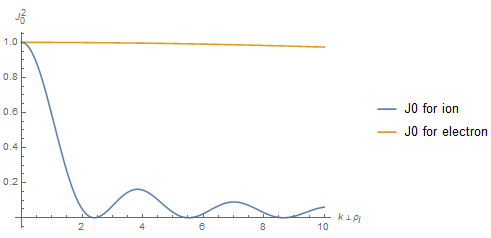
\includegraphics[width=0.9\textwidth]{Image/J0_1.PNG}
        \caption{plot of $J_0^2(k_\perp\rho_i)$ different species, small $k_\perp$}
        \label{fig:J0_1}
\end{figure}

\begin{figure}[h] \centering
        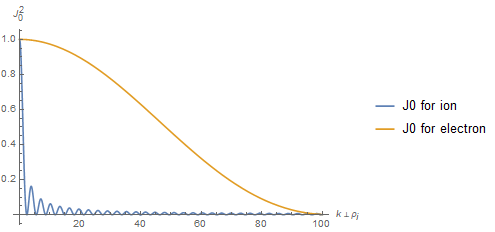
\includegraphics[width=0.9\textwidth]{Image/J0_2.PNG}
        \caption{plot of $J_0^2(k_\perp\rho_i)$ different species, large $k_\perp$}
        \label{fig:J0_2}
\end{figure}








\section{Mode induction}

All the modes are driven by the pressure gradient($\omega_{*}^{tot}$).


Perturbation of magnetic field induces electromagnetic mode - MTM. 

Let's first talk about the source of the perturbation. As the electrons and ions move (roughly) along the field line. Moving charge induces a magnetic field. From the large scale, the total magnetic perturbation should be small due to quasi-neutrality. 

\section{Mode stabilization}

Landau damping, magnetic shear suppression and $E\times B$ shear suppression 

\section{Transport}

The equation of the kinetic equation can be expressed in the following way. 

\begin{equation}
    \frac{\partial f}{\partial t} = \mathcal{L}[f]+\mathcal{N}[f,f]
\end{equation}

Where $\mathcal{L}[f]$ is the linear term and $\mathcal{N}[f,f]$ is the nonlinear term. 

Recall in linear theory we have 
\begin{equation}
    \frac{\partial f}{\partial t} = \mathcal{L}[f]
\end{equation}

Where $ \frac{\partial f}{\partial t} =\gamma f$, 
With the assumption of $\mathcal{L}[f] \approx \gamma f$ 

One can express the nonlinear term in the following way: 

\begin{equation}
    \mathcal{N}[f,f] = \sum_{k'} \left(k_x'k_y-k_xk_y'\right)\phi_{k'} f_{k,k'}
\end{equation}
$\mathcal{N}[f,f] \approx -\overline{k^2_\perp} f \phi$ for sure a 

At the saturation level, $\frac{\partial f}{\partial t} = 0$

Therefore $\chi \propto \phi \approx \frac{\gamma}{\overline{k^2_\perp}}$

Recall from

\begin{equation}
    Q=n\chi \nabla T
\end{equation}

Taking magnetic instabilities into account, we have $\chi \propto \phi+v_{||}A_{||} $

Qusailinear magnetic transport will be 

\begin{eqnarray}
    \int k_y \chi v^2 f dv\\
    =\int k_y \phi v^2 f dv + 
      \int k_y v_{||}A_{||} v^2 f dv\\
    =v_{E\times B} \delta P
    +\delta B_x q_{|| e}
\end{eqnarray}

The flaw of this model is that, linear term only considers the on mode. 

\section{Parity}

Kinetic instibilities and MHD type instabilities. For kinetic instabilities, the distribution depends on frequncy, hence the plasma with different velocity responds to different frequency. 

\textbf{Tearing parity and Ballooning parity are two eigen-solution to a $2_{nd}$ order differential equation.} Tearing being odd in $\phi$ and Ballooning being even in $\phi$. From the equation 33-39 of \cite{tearing_parity}, the mathematical aspect of the parity has been illustrated. As we know, any function can be expressed in one even function add another odd function. The even and odd function will represent different type of instabilities with different physics

In general, the differential equations can be expressed as:

\begin{eqnarray}
    \mathcal{L}(x) f(x)=0 \\
    \left[\mathcal{L}_{even}(x)+\mathcal{L}_{odd}(x)\right]f(x)=0 
    \label{eq:lxfx}
\end{eqnarray}

Where the $\mathcal{L}(x)$ is a linear operator, $\mathcal{L}(x)$ has a odd and even part $\mathcal{L}(x)=\mathcal{L}_{even}(-x)-\mathcal{L}_{odd}(-x)$. So the we have

\begin{equation}
    \left[\mathcal{L}_{even}(-x)-\mathcal{L}_{odd}(-x)\right]f(x)=0
\end{equation}

Equivalently, changing $x$ to $-x$

\begin{equation}
    \left[\mathcal{L}_{even}(x)-\mathcal{L}_{odd}(x)\right]f(-x)=0 
    \label{eq:lxf-x}
\end{equation}

Combine Equation \ref{eq:lxfx} and Equation \ref{eq:lxf-x}. Then we will have,

\begin{eqnarray}
    \mathcal{L}_{even}(x) \left[\frac{f(x) + f(-x)}{2}\right]=0\\
    \mathcal{L}_{odd}(x)  \left[\frac{f(x) - f(-x)}{2}\right]=0
\end{eqnarray}

Where $\left[\frac{f(x) + f(-x)}{2}\right]$ is a general expression of even function. On the other hand, $\left[\frac{f(x) - f(-x)}{2}\right]$ is odd. 

For two coupled differential equations

\begin{eqnarray}
    \mathcal{L}_1(x) \phi(x)=g(x)\psi(x)\\
    \mathcal{L}_2(x) \psi(x)=h(x)\phi(x)
\end{eqnarray}

If the $g(x)$ and $h(x)$ are odd, meanwhile $\mathcal{L}_1$ and $\mathcal{L}_2$ are even. Similar to previous case

\begin{eqnarray}
    \mathcal{L}_1(x) \phi(-x)=-g(x)\psi(-x)\\
    \mathcal{L}_2(x) \psi(-x)=-h(x)\phi(-x)
\end{eqnarray}

If the $\phi(x)$ is even

\begin{eqnarray}
    \mathcal{L}_1(x) \phi(x)=-g(x)\psi(-x)\\
    \mathcal{L}_2(x) \psi(-x)=-h(x)\phi(x)
\end{eqnarray}

Then $\psi(s)$ has to be odd. 

\begin{eqnarray}
    \mathcal{L}_1(x) \phi(x)=g(x)\psi(x)\\
    \mathcal{L}_2(x) \psi(x)=h(x)\phi(x)
\end{eqnarray}

Similarly, we will have the case where $\phi(x)$ is odd and $\psi(x)$ is even. 

From \cite{parity} Figure \ref{fig:parity} 

\begin{figure}[h] \centering
        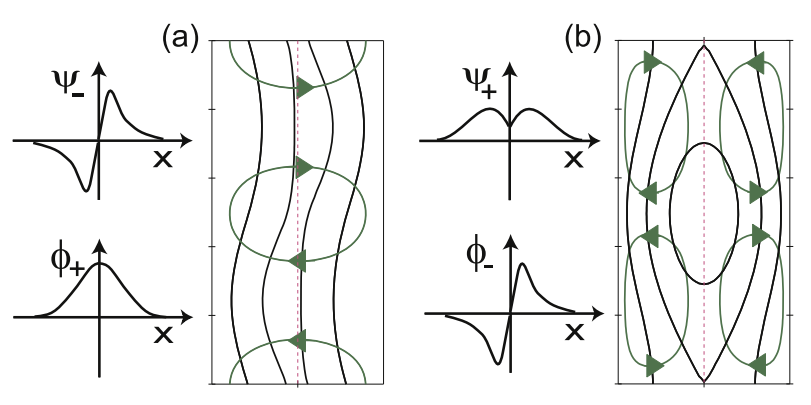
\includegraphics[width=1\textwidth]{Image/Parity.png}
        \caption{Figure7 from \cite{parity}. Electrostatic potential $\phi$ and perturbed magnetic flux $\psi$ profiles of (a) twisting parity mode $\left(\phi_{+}, \psi_{-}\right)$ and (b) tearing parity $\operatorname{mode}\left(\phi_{-}, \psi_{+}\right)$ in a slab plasma.}
        \label{fig:parity}
\end{figure}


\subsection{Ballooning parity}
\subsection{Tearing parity}

The $A_{||}$ being even around rational surface will provide the structure like olive. 